% This is part of Mes notes de mathématique
% Copyright (c) 2011-2013,2016
%   Laurent Claessens
% See the file fdl-1.3.txt for copying conditions.


%+++++++++++++++++++++++++++++++++++++++++++++++++++++++++++++++++++++++++++++++++++++++++++++++++++++++++++++++++++++++++++
\section{Théorèmes de Sylow}
%+++++++++++++++++++++++++++++++++++++++++++++++++++++++++++++++++++++++++++++++++++++++++++++++++++++++++++++++++++++++++++

\begin{lemma}
    Soient \( H\) et \( K\) des sous-groupes finis de \( G\). Alors
    \begin{equation}
        \Card(HK)=\frac{ | H |\cdot | K | }{ | H\cap K | }.
    \end{equation}
\end{lemma} 
Attention : dans ce lemme, l'ensemble \( HK\) n'est pas spécialement un groupe. Ce serait le cas si \( H\) normaliserait \( K\), c'est à dire si nous avions \( hkh^{-1}\in K<,\forall h,k\in H\times K\).

\begin{theorem}[Théorème de Cauchy]\index{Cauchy!théorème}\index{théorème!Cauchy}       \label{ThoCauchyGpFini}
    Soit \( G\) un groupe fini et \( p\) un nombre premier divisant \( | G |\). Alors 
    \begin{enumerate}
        \item
            \( G\) contient un élément d'ordre \( p\).  
        \item
            Si \( G\) est un \( p\)-groupe, il existe un élément central d'ordre \( p\) dans \( G\).
    \end{enumerate}
\end{theorem}
Une preuve du premier point est sur \wikipedia{fr}{Théorème_de_Cauchy_(groupes)}{wikipedia}.

\begin{lemma}[Théorème de Cayley]    \label{ThoIfdlEB}   \index{Cayley!théorème}
    Si \( G\) est un groupe d'ordre \( n\) alors il est isomorphe à un sous-groupe du groupe symétrique \( S_n\).
\end{lemma}

\begin{proof}
    L'action à gauche de \( G\) sur lui-même
    \begin{equation}
        \begin{aligned}
            \varphi\colon G&\to S_n \\
            \varphi(x)g&\mapsto xg 
        \end{aligned}
    \end{equation}
    est une permutation des éléments de \( G\). Cela donne un morphisme injectif parce que si \( \varphi(x)=\varphi(y)\) nous avons \( xg=yg\) pour tout \( g\) et en particulier pour \( g=e\) nous trouvons \( x=y\).
\end{proof}

\begin{lemma}       \label{LemaQxjcm}
    Soit \( p\) un diviseur premier de \( n\). Alors le groupe symétrique \( S_n\) se plonge dans \( \GL_n(\eF_p)\).
\end{lemma}

\begin{proof}
    Soit \( \{ e_i \}\) la base canonique de \( \eF_p\). Nous avons le morphisme injectif $\varphi\colon S_n\to \GL(n,\eF)$ donné par \( \varphi(\sigma)e_i=e_{\sigma(i)}\).
\end{proof}
 
\begin{remark}  \label{RemFzxxst}
    En mettant bout à bout les lemmes \ref{ThoIfdlEB} et \ref{LemaQxjcm}, nous trouvons que si \( p\) est un diviseur premier de \( | G |\), alors \( G\) peut être vu comme un sous-groupe de \( \GL(n,\eF_p)\).
\end{remark}

\begin{definition}
    Soit \( p\) un nombre premier. Un \defe{$p$-groupe}{$p$-groupe}\index{groupe!$p$-groupe} est un groupe dont tous les éléments sont d'ordre \( p^m\) pour un certain \( m\) (dépendant de l'élément).

    Soit \( G\) un groupe fini et \( p\), un diviseur premier de $| G |$. Un \defe{\(p\)-Sylow}{$p$-Sylow}\index{Sylow!$ p$-Sylow} dans \( G\) est un \( p\)-sous-groupe d'ordre \( p^n\) où \( p^n\) est la plus grande puissance de \( p\) divisant \( | G |\).
\end{definition}
Notons que si \( p\) est un nombre premier, alors tout groupe d'ordre \( p^m\) est un \( p\)-groupe.

\begin{lemma}
    Soit \( G\) un groupe fini et \( P\), \( Q\) des \( p\)-sous-groupes. Nous supposons que \( Q\) normalise \( P\). Alors \( PQ\) est un \( p\)-sous-groupe de \( G\).
\end{lemma}

Si \( S\) est un \( p\)-Sylow, alors \( p\) ne divise pas le nombre \( | G:S |=| G |/| S |\).

\begin{proposition}     \label{Propvocmon}
    Soit le corps fini \( \eF_p=\eZ/p\eZ\) (\( p\) premier). Soit \( T\) le sous-ensemble de \( \GL_n(\eF_p)\) formé des matrices triangulaires supérieures de rang\footnote{Définition \ref{DefALUAooSPcmyK}.} \( n\) et dont les éléments diagonaux sont \( 1\). Alors \( T\) est un \( p\)-Sylow de \( \GL_n(\eF_p)\).
\end{proposition}

\begin{proof}
    Nous commençons par étudier le cardinal de \( \GL_n(\eF_p)\). Pour la première colonne, la seule contrainte à vérifier est qu'elle ne soit pas nulle. Il y a donc \( p^n-1\) possibilités. Pour la seconde, il faut ne pas être multiple de la première. Il y a donc \( p^n-p\) possibilités (parce qu'il y a \( p\) multiples possibles de la premières colonne). Pour la \( k\)-ième colonne, il faut éviter toutes les combinaisons linéaires des \( (k-1)\) premières colonnes. Il y a \( p^{k-1}\) telles combinaisons et donc \( p^n-p^{k-1}\) possibilités pour la \( k\)-ième colonne. Nous avons donc
    \begin{subequations}
        \begin{align}
            \Card\big( \GL(n,\eF_{p}) \big)&=(p^n-1)(p^n-p)\ldots(p^n-p^{n-1})\\
            &=p\cdot p^2\cdots p^{n-1}(p^n-1)(p^{n-1}-1)\ldots (p-1)\\
            &=p^{\frac{ n(n-1) }{2}}m
        \end{align}
    \end{subequations}
    où \( m\) est un entier qui ne divise pas \( p\).

    En ce qui concerne le cardinal de \( T\), le calcul est plus simple : pour la première ligne nous avons \( p^{n-1}\) choix (parce qu'il y a un \( 1\) qui est imposé sur la diagonale), pour la seconde \( p^{n-2}\), etc. En tout nous avons alors
    \begin{equation}
        | T |=p^{\frac{ n(n-1) }{2}},
    \end{equation}
    et \( T\) est un \( p\)-Sylow de \( \GL_n(\eF_p)\).
\end{proof}


\begin{proposition}
    Soit \( p\) un nombre premier. Un groupe fini \( G\) est un $p$-groupe si et seulement l'ordre de \( G\) est \( p^n\) pour un certain \( n\).
\end{proposition}

\begin{proof}
    Supposons que \( G\) est un $p$-groupe. Soit \( q\) un nombre premier divisant \( | G |\). Par le théorème de Cauchy (\ref{ThoCauchyGpFini}), le groupe \( G\) contient un élément d'ordre \( q\), soit \( g\) un tel élément. Étant donné que \( G\) est un $p$-groupe, \( g^{p^n}=g^q=e\) pour un certain \( n\). Donc $q=p^n$ et \( q=p\) parce que \( q\) est premier. Nous venons de prouver que \( p\) est le seul nombre premier qui divise \( | G |\). L'ordre de \( G\) est par conséquent une puissance de \( p\).

    Nous nous intéressons maintenant à l'implication inverse. Nous supposons que \( | G |=p^n\) pour un certain entier \( n\geq 0\). Soit \( g\in G\); nous notons \( r\) l'ordre de \( G\). Le sous-groupe \( \gr(g)\) est d'ordre \( r\), donc \( r\) divise \( | G |\) (par le théorème \ref{ThoLagrange} de Lagrange). Le nombre \( r\) est alors une puissance de \( p\).
\end{proof}

\begin{lemma}       \label{LemwDYQMg}
    Soit \( G\), un groupe fini de cardinal \( | G |=n\) et \( p\), un diviseur premier de \( n\). Nous notons \( n=p^m\cdot r\) où \( p\) ne divise pas \( r\). Soit \( H\) un sous-groupe de \( G\) et \( S\), un \( p\)-Sylow de \( G\). Alors il existe \( g\in G\) tel que 
    \begin{equation}
        gSg^{-1}\cap H
    \end{equation}
    soit un \( p\)-Sylow de \( H\).
\end{lemma}

\begin{proof}
    Nous considérons l'ensemble \( G/S\) sur lequel \( H\) agit. Si \( a\in G\), le stabilisateur de \( [a]\) dans \( G/S\) est
    \begin{subequations}
        \begin{align}
            \Stab\big( [a] \big)&=\{ h\in H\tq [ha]=[a] \}\\
            &=\{ h\in H\tq a^{-1}ha\in S\}\\
            &=aSa^{-1}\cap H.
        \end{align}
    \end{subequations}
    Nous cherchons \( a\in G\) tel que l'entier
    \begin{equation}        \label{EqZpUbWx}
        \frac{ \Card(H) }{ \Card\big( aSa^{-1}\cap H \big) }
    \end{equation}
    soit premier avec \( p\). En effet, dans ce cas le groupe \( \Stab([a])\) est un $p$-Sylow de \( H\) parce que \( | H:aSa^{-1}\cap H |\) ne divise pas \( p\). La formule des orbites (équation \eqref{EqCewSXT}) nous dit que
    \begin{equation}
        \frac{ | H | }{ | aSa^{-1}\cap H | }=\Card\big( \mO_{[a]} \big).
    \end{equation}
    Supposons que toutes les orbites aient un cardinal divisible par \( p\). Étant donné que \( G/S\) est une réunion disjointe de ses orbites, nous aurions
    \begin{equation}
        p\divides \Card(G/S)=\frac{ | G | }{ | S | }
    \end{equation}
    alors que \( S\) étant un $p$-Sylow, \( p\) ne peut pas diviser \( | G |/| S |\). Toutes les orbites n'ont donc pas un cardinal divisible par \( p\), et il existe un \( a\in G\) tel que \eqref{EqZpUbWx} soit vérifiée.
\end{proof}


\begin{theorem}[Théorème de Sylow]  \label{ThoUkPDXf}
    Soit \( G\) un groupe fini et \( p\), un diviseur premier de \( | G |\). Alors
    \begin{enumerate}
        \item
            \( G\) possède des \( p\)-Sylow.
        \item
            Tout \( p\)-sous-groupe de \( G\) est contenu dans un \( p\)-Sylow.
        \item   \label{ItemMzNRVf}
            Les \( p\)-Sylow de \( G\) sont conjugués.
        \item   \label{ItemkYbdzZ}
            Si \( n_p\) est le nombre de $p$-Sylow de \( G\), alors \( n_p\) divise \( | G |\) et \( n_p\equiv 1\mod p\).
    \end{enumerate}
\end{theorem}
\index{groupe!fini}

\begin{proof}

    % Il y a ici un début d'une preuve qui fonctionne d'une autre manière. Dans cette démonstration, N est l'ordre de G.

    %\begin{enumerate}
        %\item
         %   Nous faisons la récurrence sur l'ordre \( N\) de \( G\). Pour \( N=1\), le seul \( p\)-Sylow est le groupe entier. Si \( N>1\), nous commençons par supposer que \( G\) contient un sous-groupe propre \( H\) tel que \( \pgcd(| G:H |,p)=1\).
%
 %           Si \( G\) contient un sous-groupe propre \( H\) tel que \( \pgcd(| G:H |,p)=1\), alors \( p\) divise \( | G:H |\). En effet \( p\) divise \( N\) et \( | G:H |=| G |/| H |\). Si il n'y a pas de \( p\) dans la décomposition de \( | H |\), alors \( p\) divise encore \( | G |/| H |\). Étant donné que \( p\) est un diviseur premier de \( | H |\), le groupe \( H\) contient des \( p\)-Sylow par hypothèse de récurrence. Montrons que si \( S\) est un \( p\)-Sylow de \( H\), alors \( S\) est également un $p$-Sylow de \( G\).
%
 %           Soit \( S\), un $p$-Sylow de \( H\). Nous avons \( | S |=p^n\) où \( n\) est la plus grande puissance de \( p\) divisant \( H\). Par hypothèse, il n'y a pas de \( p\) dans la décomposition de \( | G:H |\); par conséquent \( p^n\) est également la plus grande puissance de \( p\) qui divise \( | G |\) et \( S\) est alors un $p$-Sylow de \( G\).
%
 %           Nous supposons maintenant que \( G\) ne possède pas de sous-groupe \( H\) tels que \( \pgcd(| G:H |,p)=1\).
%
 %   \end{enumerate}

    \begin{enumerate}
        \item
            
            Nous savons de la remarque \ref{RemFzxxst} que \( G\) est un sous-groupe de \( \GL_n(\eF_p)\) et que ce dernier a un $p$-Sylow par la proposition \ref{Propvocmon}. Par conséquent \( G\) possède un $p$-Sylow par le lemme \ref{LemwDYQMg}.

        \item

            Soit \( H\) un \( p\)-sous-groupe de \( G\) et \( S\), un $p$-Sylow de \( G\) (qui existe par le point précédent). Par le lemme \ref{LemwDYQMg} il existe \( a\in G\) tel que \( aSa^{-1}\cap H\) soit un $p$-Sylow de \( H\). Mais \( H\) est un \(p\)-groupe et un $p$-Sylow dans un \( p\)-groupe est automatiquement le groupe entier. Par conséquent,
            \begin{equation}
                H=aSa^{-1}\cap H
            \end{equation}
            et \( H\subset aSa^{-1}\), ce qui signifie que \( H\) est inclus à un $p$-Sylow.

        \item

            Soit \( H\) un $p$-Sylow. Nous venons de voir que si \( S\) est un $p$-Sylow quelconque, alors \( H\) est inclus au $p$-Sylow \( aSa^{-1}\) pour un certain \( a\in G\). Donc \( H\) est un $p$-Sylow inclus dans le $p$-Sylow \( aSa^{-1}\), donc \( H=aSa^{-1}\).

        \item

            Le fait que \( n_p\) divise \( n\) est parce que tous les $p$-Sylow ont le même nombre d'éléments (ils sont conjugués) et sont deux à deux disjoints. Donc ils forment une partition de \( G\) et \( | G |=n_p| S |\) si \( S\) est un $p$-Sylow quelconque.
            
            Montrons maintenant que \( n_p\) est congru à un modulo \( p\). Soit \( E\) l'ensemble des $p$-Sylow de \( G\). Le groupe \( G\) agit sur \( E\) par conjugaison. Soit \( S\) un $p$-Sylow et considérons l'ensemble
            \begin{equation}
                E_S=\{ T\in E\tq s\cdot T=T\forall s\in S \}.
            \end{equation}
            où l'action est celle par conjugaison. C'est l'ensemble des points fixes de \( E\) sous l'action de \( S\). L'ensemble \( E\) est la réunion des orbites sous \( S\) et chacune de ces orbites a un cardinal qui divise \( | S |=p^m\). Par conséquent \( | \mO_T |\) vaut \( 1\) lorsque \( T\in E_S\) et est un multiple de \( p\) sinon. Nous avons donc
            \begin{equation}
                | E |\equiv | E_S |\mod p.
            \end{equation}
            Nous voulons obtenir \( | E_S |=1\). Évidemment \( S\in E_S\) parce que si \( s\in S\) alors \( sSs^{-1}=S\). Nous voudrions montrer que \( S\) est le seul élément de \( E_S\). Soit \( T\in E_S\), c'est à dire que \( T\) est un $p$-Sylow de \( G\) tel que
            \begin{equation}
                sTs^{-1}=T
            \end{equation}
            pour tout \( s\in S\). Soit \( N\) le groupe engendré par \( S\) et \( T\). Montrons que \( T\) est normal dans \( N\). Un élément \( g\) dans \( N\) s'écrit
            \begin{equation}
                g=s_1t_1\cdots s_rt_r
            \end{equation}
            avec \( s_i\in S\) et \( t_i\in T\). Si \( t\in T\), en utilisant le fait que \( T\) est un groupe et le fait que \( S\) le normalise, nous avons
            \begin{equation}
                gtg^{-1}=s_1t_1\ldots s_rt_rtt_r^{-1}s_r^{-1}\ldots t_1^{-1}s_r^{-1}\in T.
            \end{equation}
            Donc \( T\) est un sous-groupe normal de \( N\). Mais \( S\) et \( T\) sont conjugués dans \( N\) (parce que ils sont des $p$-Sylow de \( N\)), donc il existe un élément \( a\in N\) tel que \( aTa^{-1}=S\). Mais étant donné que \( T\) est normal,
            \begin{equation}
                S=aTa^{-1}=T.
            \end{equation}
            Ceci achève la démonstration des théorèmes de Sylow.

    \end{enumerate}
\end{proof}

\begin{proposition}
    Si \( S\) est un \( p\)-Sylow dans le groupe \( G\) alors pour tout \( g\in G\), l'ensemble \( gSg^{-1}\) est encore un \( p\)-groupe.    
\end{proposition}

\begin{proof}
    Si les éléments de \( S\) sont d'ordre \( p^n\), alors nous avons
    \begin{equation}
        (gsg^{-1})^q=gs^qg^{-1}=e.
    \end{equation}
    Pour avoir \( gs^qg^{-1}=e\), il faut et suffit que \( gs^q=g\), alors \( s^q=e\), c'est à dire \( q=p^n\). Donc \( gSg^{-1}\) est encore un \( p\)-Sylow.
\end{proof}

Les deux résultats \ref{Lemcmbzum} et \ref{PropyfhTmf} proviennent de la \wikiversity{fr}{Groupe_(mathématiques)/Exercice/Premiers_résultats_sur_les_groupes_simples}{wikiversité}.
\begin{lemma}\label{Lemcmbzum}
    Soit \( G\), un groupe fini et \( p\), un nombre premier. Si \( H\) et \( K\) sont des groupes distincts d'ordre \( p\), alors \( H\cap K=\{ e \}\).
\end{lemma}

\begin{proof}
    L'ensemble \( H\cap K\) est un sous-groupe de \( H\). Par conséquent son ordre divise celui de \( H\) qui est un nombre premier. Par conséquent soit \( | H\cap K |=1\), soit \( | H\cap K |=| H |\). Dans le second cas nous aurions \( H=K\), alors que nous avons supposé que \( H\) et \( K\) étaient distincts.
\end{proof}

\begin{proposition} \label{PropyfhTmf}
    Soit \( G\) un groupe fini et \( n\) le nombre de sous-groupes d'ordre \( p\) dans \( G\). Alors le nombre d'éléments d'ordre \( p\) dans \( G\) vaut \( n(p-1)\).
\end{proposition}

\begin{proof}
    Si \( g\) est un élément d'ordre \( p\) dans \( G\), le groupe \( H\) engendré par \( g\) est d'ordre \( p\). Réciproquement si \( H\) est un groupe d'ordre \( p\), tous les éléments de \( H\setminus\{ e \}\) sont d'ordre \( p\) (parce que l'ordre d'un élément divise l'ordre du groupe). Donc l'ensemble des éléments d'ordre \( p\) dans \( G\) est la réunion des ensembles \( H\setminus\{ e \}\) où \( H\) parcours les sous-groupes d'ordre \( p\) dans \( G\). Chacun de ces ensembles possède \( p-1\) éléments et le lemme \ref{Lemcmbzum} nous assure qu'ils sont disjoints. Par conséquent nous avons \( n(p-1)\) éléments d'ordre \( p\) dans \( G\).
\end{proof}

\begin{corollary}
    Un groupe d'ordre premier est cyclique.
\end{corollary}

\begin{proof}
    Soit \( p\) l'ordre de \( G\). Le nombre de sous-groupes d'ordre \( p\) est \( n=1\) (et c'est \( G\) lui-même). La proposition \ref{PropyfhTmf} nous dit alors que le nombre d'éléments d'ordre \( p\) dans \( G\) est \( p-1\). Donc tout élément est générateur.
\end{proof}

\begin{lemma}
    Le groupe \( A_6\) n'accepte pas de sous-groupes normaux d'ordre \( 60\).
\end{lemma}

\begin{proof}
    Soit \( G\) normal dans \( A_6\), et \( a\), un élément d'ordre \( 5\) dans \( G\) (qui existe parce que \( 5\) divise \( 60\)). Soit aussi un élément \( b\) d'ordre \( 5\) dans \( A_6\). Les groupes \( \gr(a)\) et \( \gr(b)\) sont deux \( 5\)-Sylow dans \( A_6\). En effet, \( 5\) un nombre premier et est la plus grande puissance de \( 5\) dans la décomposition de \( 60\); donc \( \gr(a)\) est un \( 5\)-Sylow dans \( G\). D'autre part, l'ordre de \( A_6\) (qui est \( \frac{ 1 }{2}6!\)) ne possède également que \( 5\) à la puissance \( 1\) dans sa décomposition.

    En vertu du théorème de Sylow \ref{ThoUkPDXf}\ref{ItemMzNRVf}, les \( 5\)-Sylow \( \gr(a)\) et \( \gr(b)\) sont conjugués et il existe \( \tau\in A_6\) tel que \( b=\tau a\tau^{-1}\). Mais \( G\) étant normal dans \( A_6\), l'élément \( \tau a\tau^{-1}\) est encore dans \( G\), de telle sorte que \( b\in G\). Du coup \( G\) doit contenir tous les éléments d'ordre \( 5\) de \( A_6\).

    Les éléments d'ordre $5$ de \( A_6\) doivent fixer un des points de \( \{ 1,2,3,4,5,6 \}\) puis permuter les autres de façon à n'avoir qu'un seul cycle. Un cycle correspond à écrire les nombres \( 1,2,3,4,5\) dans un certain ordre. Ce faisant, le premier n'a pas d'importance parce qu'on considère la permutation cyclique, par exemple \( (3,5,2,1,4)\) est la même chose que \( (5,2,1,4,3)\). Le nombre de cycles sur \( \{ 1,2,3,4,5 \}\) est donc de \( 4!\), et par conséquent le nombre d'éléments d'ordre \( 5\) dans \( A_6\) est \( 6\cdot 4!=144\).

    Le groupe \( G\) doit contenir au moins \( 144\) éléments alors que par hypothèse il en contient \( 60\); contradiction.
    
\end{proof}

\begin{proposition}[\cite{Exo7Sylow}]
    Tout groupe simple d'ordre \( 60\) est isomorphe au groupe alterné \( A_5\).
\end{proposition}
Une autre preuve de ce résultat peut être trouvée sur la \wikiversity{fr}{Groupe_(mathématiques)/Exercice/Premiers_résultats_sur_les_groupes_simples}{wikiversité}. 

\begin{proof}
    Nous avons la décomposition en nombres premiers \( 60=2^2\cdot 3\cdot 5\). Déterminons pour commencer le nombre \( n_5\) de \( 5\)-Sylow dans \( G\). Le théorème de Sylow \ref{ThoUkPDXf}\ref{ItemkYbdzZ} nous renseigne que \( n_5\) doit diviser \( 60\) et doit être égal à \( 1\mod 5\). Les deux seules possibilités sont \( n_5=1\) et \( n_5=6\). Étant donné que tous les \( p\)-Sylow sont conjugués, si \( n_5=1\) alors le \( 5\)-Sylow serait un sous-groupe invariant à l'intérieur de $G$, ce qui est impossible vu que \( G\) est simple. Donc \( n_5=6\).

    Par le point \ref{ItemMzNRVf} du théorème de Sylow, le groupe \( G\) agit transitivement sur l'ensemble des \( 5\)-Sylow par l'action adjointe :
    \begin{equation}
        g\cdot S=gSg^{-1}.
    \end{equation}
    Cela donne donc un morphisme \( \theta\colon G\to S_6\). Le noyau de \( \theta\) est un sous-groupe normal. En effet si \( k\in \ker\theta\) et si \( g\in G\) nous avons
    \begin{subequations}
        \begin{align}
            (gkg^{-1})\cdot S&=gkg^{-1} Ggk^{-1}g^{-1}\\
            &=gkTk^{-1}g^{-1}\\
            &=gTg^{-1}\\
            &=S
        \end{align}
    \end{subequations}
    où \( T\) est le Sylow \( T=g^{-1}Sg\). Étant donné que \( k\in \ker\theta\) nous avons utilisé \( kTk^{-1}=aT\). Au final \( gkg^{-1}\cdot S=S\), ce qui prouve que \( gkg^{-1} \in\ker\theta\).

    Étant donné que \( \ker\theta\) est normal dans \( G\), soit est soit réduit à \( \{ e \}\) soit il vaut \( G\). La seconde possibilité est exclue parce qu'elle reviendrait à dire que \( G\) agit trivialement, ce qui n'est pas correct étant donné qu'il agit transitivement. Nous en déduisons que \( \ker\theta=\{ e \}\), que \( \theta\) est injective et que \( G\) est isomorphe à un sous-groupe de \( S_6\).

    Par ailleurs le groupe dérivé de \( G\) est un sous-groupe normal (et non réduit à l'identité parce que \( G\) est non commutatif). Donc \( D(G)=G\). Étant donné que \( G\subset S_6\), nous avons
    \begin{equation}
        G=D(G)\subset D(S_6)=A_6
    \end{equation}
    parce que le groupe dérivé du groupe symétrique est le groupe alterné (lemme \ref{LemiApyfp}).

    L'ensemble \( \theta^{-1}(A_6)\) est distingué dans \( G\). En effet si \( \sigma\in A_6\) et si \( g\in G\) nous avons
    \begin{equation}
        \theta\big( g\theta^{-1}(\sigma)g^{-1} \big)=\theta(g)\sigma \theta(g)^{-1}\in A_6.
    \end{equation}
    Nous en déduisons que \( \theta^{-1}(A_6)\) est soit \( G\) entier soit réduit à \( \{ e \}\). Si \( \theta^{-1}(A_6)=\{ e \}\), alors pour tout \( g\in G\) nous aurions \( g^2=e\) parce que \( \theta(g^2)\in A_6\). L'ordre de \( G\) étant \( 60\), il n'est pas possible que tous ses éléments soient d'ordre \( 2\). Nous en déduisons que \( \theta(G)\subset A_6\).

    Nous nommons \( H=\theta(G)\) et nous considérons l'ensemble \( X=A_6/H\) où les classes sont prises à gauche, c'est à dire 
    \begin{equation}
        [\sigma]=\{ h\sigma\tq h\in H \}.
    \end{equation}
    Évidemment \( A_6\) agit sur \( X\) de façon naturelle. Au niveau de la cardinalité,
    \begin{equation}
        \Card(X)=\frac{ | A_6 | }{ | G | }=\frac{ 360 }{ 60 }=6.
    \end{equation}
    Le groupe \( A_6\) agit sur \( X\) qui a \( 6\) éléments. Nous avons donc une application \( \varphi\colon A_6\to A_6\). Encore une fois, la simplicité de \( A_6\) montre que \( \varphi(A_6)=A_6\).

    Nous étudions maintenant \( \varphi(H)\) agissant sur \( X\). Un élément \( x\in A_6\) fixe la classe de l'unité \( [e]\) si et seulement si \( x\in H\) et par conséquent \( \varphi(H)\) est la fixateur de \( [e]\) dans \( X\). À la renumérotation près, nous pouvons identifier \( \varphi(H)\) au sous-groupe de \( A_6\) agissant sur \( \{ 1,\ldots, 6 \}\) et fixant \( 6\). Nous avons alors \( \varphi(H)=S_5\cap A_6=A_5\). Nous venons de prouver que \( \varphi\) fournit un isomorphisme entre \( A_5\) et \( H\). Étant donné que \( H\) était isomorphe à \( G\), nous concluons que \( G\) est isomorphe à \( A_6\).
\end{proof}

%+++++++++++++++++++++++++++++++++++++++++++++++++++++++++++++++++++++++++++++++++++++++++++++++++++++++++++++++++++++++++++
\section{Un peu de classification de groupes}
%+++++++++++++++++++++++++++++++++++++++++++++++++++++++++++++++++++++++++++++++++++++++++++++++++++++++++++++++++++++++++++

\begin{definition}
    Un \defe{nombre premier}{nombre!premier} est un naturel acceptant exactement deux diviseurs distincts.
\end{definition}
Avec cette définition, \( 0\) n'est pas premier, \( 1\) n'est pas premier et \( 2\) est premier.

%---------------------------------------------------------------------------------------------------------------------------
\subsection{Automorphismes du groupe \texorpdfstring{$ \eZ/n\eZ$}{Z/nZ}}
%---------------------------------------------------------------------------------------------------------------------------

Notons que \( \eZ/n\eZ=\eZ/n\eZ=\eF_n\) est un groupe pour l'addition tandis que \( (\eZ/n\eZ)^*\) est un groupe pour la multiplication. Il ne peut donc pas y avoir d'équivoque.

\begin{theorem}[\href{https://fr.wikiversity.org/wiki/Groupe\_\%28math\%C3\%A9matiques\%29/Automorphismes\_d'un\_groupe\_cyclique}{Wikiversité}%
    ]   \label{ThoozyeSn}
    Pour chaque \( x\in (\eZ/n\eZ)^*\) nous considérons l'application
    \begin{equation}
        \begin{aligned}
            \sigma_x\colon \eZ/n\eZ&\to \eZ/n\eZ \\
            y&\mapsto xy. 
        \end{aligned}
    \end{equation}
    L'application
    \begin{equation}
        \sigma\colon \big( (\eZ/n\eZ)^*,\cdot\big)\to \Aut\big( \eZ/n\eZ,+ \big)
    \end{equation}
    ainsi définie est un isomorphisme de groupes.
\end{theorem}
L'énoncé de ce théorème s'écrit souvent rapidement par 
\begin{equation}
    \Aut(\eZ/n\eZ)=(\eZ/n\eZ)^*,
\end{equation}
mais il faut bien garder à l'esprit qu'à gauche on considère le groupe additif et à droite celui multiplicatif.

\begin{proof}
    Nous notons \( [x]\) la classe de \( x\) dans \( \eZ/n\eZ\). Nous avons \( \eZ/n\eZ=[1]\). Soit \( f\) un automorphisme de \( (\eZ/n\eZ,+)\); pour tout \( r\in \eZ\) nous avons
    \begin{equation}
        f([r])=f(r[1])=rf([1])=[r]f([1]).
    \end{equation}
En particulier, vu que \( f\) est surjective, il existe un \( r\) tel que \( f([r])=[1]\). Pour un tel \( r\) nous avons \( [1]=[r]f([1])\), c'est à dire que nous avons montré que \( f([1])\) est inversible dans \(  \big( (\eZ/n\eZ)^*,\cdot\big)\). Nous montrons à présent que\footnote{Le \( \sigma\) donné ici est l'inverse de celui donné dans l'énoncé. Cela ne change évidemment rien à la validité de l'énoncé et de la preuve.}
    \begin{equation}
        \begin{aligned}
            \sigma\colon \Aut( (\eZ/n\eZ,+))&\to \big( (\eZ/n\eZ)^*,\cdot \big)<++>\\
            f&\mapsto f([1]) 
        \end{aligned}
    \end{equation}
    est un isomorphisme.

    Nous commençons par la surjectivité. Soit \( [a]\in (\eZ/n\eZ)^*\). Les élément \( [a]\) et \( [1]\) étant tous deux des générateurs de \( (\eZ/n\eZ,+)\), il existe un automorphisme de \( \eZ/n\eZ\) qui envoie \( [1]\) sur \( [a]\) par le lemme \ref{LemZhxMit}. Cela prouve la surjectivité de \( \sigma\).

    En ce qui concerne l'injectivité, considérons \( f_1\) et \( f_2\) sont de automorphismes de \( (\eZ/n\eZ,+)\) tels que \( f_1([1])=f_2([1])\). Les automorphismes \( f_1\) et \( f_2\) prennent la même valeur sur un générateur et donc sur tout le groupe. Donc \( f_1=f_2\).

    Enfin nous prouvons que \( \sigma\) est un morphisme, c'est à dire que \( \sigma(f\circ g)=\sigma(f)\sigma(g)\). Nous avons
    \begin{subequations}
        \begin{align}
            f\big( g([1]) \big)&=f\big( g([1])[1j] \big)=g([1])f([1])=\sigma(f)\sigma(g).
        \end{align}
    \end{subequations}
\end{proof}

Ce dernier résultat s'étend aux groupes cycliques.
\begin{proposition}
    Si \( G\) est un groupe cyclique d'ordre \( n\), alors
    \begin{equation}
        \Aut(G)=(\eZ/n\eZ)^*.
    \end{equation}
\end{proposition}

\begin{corollary}       \label{CorwgmoTK}
    Si \( p\) divise \( q-1\) alors \( \Aut(\eF_q)\) possède un unique sous-groupe d'ordre \( p\).
\end{corollary}

\begin{proof}
    Si \( a\) est un générateur de \( \eF_q^*\) alors le groupe
    \begin{equation}    \label{EqAdGiil}
        \gr\left( a^{\frac{ q-1 }{ p }} \right)
    \end{equation}
    est un sous-groupe d'ordre \( p\). En ce qui concerne l'unicité, soit \( S\) un sous-groupe d'ordre \( p\). Il est donc d'indice \( (q-1)/p\) dans \( \eF_q^*\) et le lemme \ref{PropubeiGX} nous enseigne que le groupe donné en \eqref{EqAdGiil} est contenu dans \( S\). Il est donc égal à \( S\) parce qu'il a l'ordre de \( S\). Le fait que \( S\) soit normal est dû au fait que \( \eF_q^*\) est abélien.
\end{proof}

%---------------------------------------------------------------------------------------------------------------------------
\subsection{Groupes abéliens finis}
%---------------------------------------------------------------------------------------------------------------------------
 
Source : \cite{FabricegPSFinis}.

Nous rappelons que l'exposant\index{exposant} d'un groupe fini est le \( \ppcm\) des ordres de ses éléments. Dans le cas des groupes abéliens finis, l'exposant joue un rôle important du fait qu'il existe un élément dont l'ordre est l'exposant. Cela est le théorème suivant.

\begin{theorem}[Exposant dans un groupe abélien fini]
    Un groupe abélien fini contient un élément dont l'ordre est l'exposant du groupe.
\end{theorem}

\begin{proof}
    Soit \( G\) un groupe abélien fini et \( x\in G\), un élément d'ordre maximum \( m\). Nous montrons par l'absurde que l'ordre de tous les éléments de \( G\) divise \( m\). Soit donc \( y\in G\), un élément dont l'ordre ne divise pas \( m\); nous notons $q$ son ordre. Vu que \( q\) ne divise pas \( m\), le nombre \( q\) possède au moins un facteur premier plus de fois que \( m\) : soit \( p\) premier tel que la décomposition de \( q\) contienne \( p^{\beta}\) et celle de \( m\) contienne \( p^{\alpha}\) avec \( \beta>\alpha\). Autrement dit,
    \begin{subequations}
        \begin{align}
            m=p^{\alpha}m'\\
            q=p^{\beta}q'
        \end{align}
    \end{subequations}
    où \( m'\) et \( q'\) ne contiennent plus le facteur \( p\). L'élément \( x\) étant d'ordre \( m\), l'élément \( x^{p^{\alpha}}\) est d'ordre \( m'\). De la même manière, l'élément \( y^{q'}\) est d'ordre \( p^{\beta}\). Étant donné que \( p^{\beta}\) et \( m'\) sont premiers entre eux, l'élément  \( x^{p^{\alpha}}y^{q'}\) est d'ordre \( p^{\alpha}m'>m\). D'où une contradiction avec le fait que \( x\) était d'ordre maximal.

    Par conséquent l'ordre de tous les éléments de $G$ divise celui de \( x\) qui est alors le \( \ppcm\) des ordres de tous les éléments de \( G\), c'est à dire l'exposant de \( G\).
\end{proof}

\begin{proposition} \label{PropfPRVxi}
    Soit \( G\) un groupe abélien fini et \( x\in G\), un élément d'ordre maximum. Alors
    \begin{enumerate}
        \item
            Il existe un morphisme \( \varphi\colon G\to \gr(x)\) tel que \( \varphi(x)=x\).
        \item   \label{ItemKRYwjU}
            Il existe un sous-groupe \( K\) de \( G\) tel que \( G=\gr(x)\oplus K\).
    \end{enumerate}
\end{proposition}

\begin{proof}
    Nous notons \( a\) l'ordre de \( x\) qui est également l'exposant du groupe \( G\).

    Nous allons prouver la première partie par récurrence sur l'ordre du groupe. Si \( G=\gr(x)\), alors c'est évident. Soit \( H\) un sous-groupe propre de \( G\) contenant \( x\) et tel que le problème soit déjà résolu pour \( H\) : il existe un morphisme \( \varphi\colon H\to \gr(x)\) tel que \( \varphi(x)=x\). Soit \( y\in G\setminus H\), d'ordre \( b\). Nous allons trouver un morphisme $\hat\varphi\colon \gr(H,y)\to \gr(x) $ telle que \( \hat\varphi(x)=x\).

    Pour cela nous commençons par construire les applications suivantes :
    \begin{equation}
        \begin{aligned}
            \tilde \varphi\colon \eZ/b\eZ\times H&\to \gr(x) \\
            (\bar k,h)&\mapsto x^{kl}\varphi(h) 
        \end{aligned}
    \end{equation}
    où \( l\) est encore à déterminer, et
    \begin{equation}
        \begin{aligned}
            p\colon \eZ/b\eZ\times H&\to \gr(y,H) \\
            (\bar k,h)&\mapsto y^kh. 
        \end{aligned}
    \end{equation}
    Pour que \( \tilde \varphi\) soit bien définie, il faut que \( a\) divise \( bl\). L'application \( p\) est bien définie parce que \( \bar k\) est pris dans \( \eZ/b\eZ\) et que \( b\) est l'ordre de \( y\).

    Nous allons construire le morphisme \( \hat \varphi\) en considérant le diagramme 
    \begin{equation}
    \xymatrix{%
    \ker(p) \ar@{^{(}->}[r]        &   \eZ/b\eZ\times H\ar[d]_{\tilde \varphi}\ar[r]^p&\gr(y,H)\ar[ld]^{\hat \varphi}\\
          &   \gr(x)
       }
    \end{equation}
    que l'on voudra être commutatif. Vu que \( p\) est surjective, les théorèmes d'isomorphismes nous disent que
    \begin{equation}
        \gr(y,H)\simeq\frac{ \eZ/b\eZ\times H }{ \ker p }.
    \end{equation}
    Si \( [\bar k,h]\) est la classe de \( (\bar k,h)\) modulo \( \ker(p)\) alors nous voudrions définir \( \hat \varphi\) par
    \begin{equation}        \label{EqeesVxc}
        \hat\varphi\big( [\bar k,h] \big)=\tilde \varphi(\bar k,h).
    \end{equation}
    Pour que cela soit bien définit, il faut que si \( (\bar r,z)\in \ker p\),
    \begin{equation}
        \hat\varphi\big( [\bar k\bar r,hz] \big)=\hat\varphi\big( [\bar k,h] \big),
    \end{equation}
    c'est à dire que \( \tilde \varphi(\bar r,z)=e\). Du coup la définition \eqref{EqeesVxc} n'est bonne que si et seulement si
    \begin{equation}
        \ker(p)\subset\ker(\tilde\varphi ).
    \end{equation}
    Nous pouvons obtenir cela en choisissant bien \( l\).

    Déterminons d'abord le noyau de \( p\). Pour cela nous considérons un nombre \( \beta\) divisant \( b\) tel que \( \gr(y)\cap H=\gr(y^{\beta})\). Nous aurons \( p(\bar k,h)=e\) si et seulement si \( y^h=e\). En particulier \( h=y^{-k}\in\gr(y)\cap H=\gr(y^{\beta})\). Si \( h=(y^{\beta})^m=y^{m\beta}\), alors \( k=-m\beta\) et nous avons
    \begin{equation}
        \ker(p)=\{ (-m\beta,y^{m\beta})\tq m\in \eZ \}.
    \end{equation}
    En plus court : \( \ker(p)=\gr(\beta,y^{-\beta})\). Nous devons donc fixer \( l\) de telle sorte que \( \tilde \varphi(\beta,y^{-\beta})=e\). Étant donné que \( \varphi\) prend ses valeurs dans \( \gr(x)\), il existe un entier \( \alpha\) tel que \( \varphi(y^{-\beta})=x^{\alpha}\); en utilisant cet \( \alpha\), nous écrivons
    \begin{equation}
        \tilde \varphi(\beta,y^{-\beta})=x^{\beta l}\varphi(y^{-\beta})=x^{\beta l+\alpha}.
    \end{equation}
    Par conséquent nous choisissons \( l=-\alpha/\beta\). Nous devons maintenant vérifier que ce choix est légitime, c'est à dire que \( a\) divise \( bl\) et que \( \alpha/\beta\) est un entier.

    Étant donné que \( y\) est d'ordre \( b\),
    \begin{equation}
        e=\varphi(y^b)=\varphi(y^{-\beta b/\beta})=\varphi(y^{-\beta})^{b/\beta}=x^{b\beta/\alpha}.
    \end{equation}
    Par conséquent \( a\) divise \( \frac{ b\alpha }{ \beta }=-bl\).

    Pour voir que \( l\) est entier, nous nous rappelons que \( a\) est l'exposant de \( G\) (parce que \( x\) est d'ordre maximum) et que par conséquent \( b\) divise \( a\). Mais \( a\) divise \( \alpha\frac{ b }{ \beta }\). Donc \( \alpha/\beta\) est entier.

    Nous passons maintenant à la seconde partie de la preuve. Nous considérons un morphisme \( \varphi\colon G\to \gr(x)\) tel que \( \varphi(x)=x\). La première partie nous en assure l'existence. Nous montrons que 
    \begin{equation}
        \begin{aligned}
            \psi\colon G&\to \gr(x)\oplus \ker(\varphi) \\
            g&\mapsto \big( \varphi(g),g\varphi(g)^{-1} \big) 
        \end{aligned}
    \end{equation}
    est un isomorphisme. D'abord \( g\varphi(g)^{-1}\) est dans le noyau de \( \varphi\) parce que \( \varphi(g)^{-1}\) étant dans \( \gr(x)\), et \( \varphi\) étant un morphisme,
    \begin{equation}
        \varphi\big( g\varphi(g)^{-1} \big)=\varphi(g)\varphi(g)^{-1}=e.
    \end{equation}
    L'application \( \psi\) est un morphisme parce que, en utilisant le fait que \( G\) est abélien,
    \begin{subequations}
        \begin{align}
            \psi(g_1g_2)&=\big( \varphi(g_1g_2),g_1g_2\varphi(g_1g_2)^{-1} \big)\\
            &=\big( \varphi(g_1)\varphi(g_2),g_1\varphi(g_1)^{-1}g_2\varphi(g_2)^{-1} \big)\\
            &=\psi(g_1)\psi(g_2).
        \end{align}
    \end{subequations}
    L'application \( \psi\) est injective parce que si \( \psi(g)=(e,e)\) alors \( \varphi(g)=e\) et \( g\varphi(g)^{-1}=e\), ce qui implique \( g=e\).

    Enfin \( \psi\) est surjective parce qu'elle est injective et que les ensembles de départ et d'arrivée ont même cardinal. En effet par le premier théorème d'isomorphisme (théorème \ref{ThoPremierthoisomo}) appliqué à \( \varphi\) nous avons
    \begin{equation}
        | G |=| \gr(x) |\cdot | \ker(\varphi) |.
    \end{equation}
\end{proof}

\begin{theorem} \label{ThoRJWVJd}
    Tout groupe abélien fini (non trivial) se décompose en
    \begin{equation}
        G\simeq \eZ/d_1\eZ\oplus\ldots\oplus \eZ/d_r\eZ
    \end{equation}
    avec \( d_1\geq 1\) et \( d_i\) divise \( d_{i+1}\) pour tout \( i=1,\ldots, r-1\).

    De plus la liste \( (d_1,\ldots, d_r)\) vérifiant ces propriétés est unique.
\end{theorem}

\begin{proof}
    Soit \( x_1\) un élément d'ordre maximal dans \( G\). Soit \( n_1\) son ordre et
    \begin{equation}
        H_1=\gr(x_1)=\eF_{n_1}.
    \end{equation}
    D'après la proposition \ref{PropfPRVxi}\ref{ItemKRYwjU}, il existe un supplémentaire \( K_1\) tel que \( G=\eF_{n_1}\oplus K_1\). Si \( K_1=\{ 1 \}\) on s'arrête et on garde \( G=\eF_{n_1}\). Sinon on continue de la sorte en prenant \( x_2\) d'ordre maximal dans \( K_1\) etc.

    Nous devons maintenant prouver l'unicité de cette décomposition. Soit
    \begin{equation}
        G=\eF_{d_1}\oplus\ldots\oplus \eF_{d_r}=\eF_{s_1}\oplus\ldots\oplus \eF_{s_q}.
    \end{equation}
    L'exposant de \( G\) est \( d_r\) et \( s_q\). Donc \( d_r=s_q\). Les complémentaires étant égaux nous avons
    \begin{equation}
        \eF_{d_1}\oplus\ldots\oplus \eF_{d_{r-1}}=\eF_{s_1}\oplus\ldots\oplus \eF_{s_{q-1}}.
    \end{equation}
    En continuant nous trouvons \( r=q\) et \( d_i=s_i\).
\end{proof}
 
%---------------------------------------------------------------------------------------------------------------------------
\subsection{Groupes d'ordre \texorpdfstring{$ pq$}{pq}}
%---------------------------------------------------------------------------------------------------------------------------
\index{quotient!de groupes}\index{sous-groupe!normal}

Soit \( G\) un groupe d'ordre \( pq\) où \( p\) et \( q\) sont des nombres premiers distincts. Nous supposons que \( p<q\). Montrons que \( G\) ne possède qu'un seul \( q\)-Sylow. Soit \( n_q\) le nombre de \( q\)-Sylow; par les théorèmes de Sylow nous avons
\begin{equation}
    n_q=1\mod q
\end{equation}
et \( n_q\) divise \( | G |=pq\). Donc \( n_q\) vaut \( p\), \( q\) ou \( 1\). Avoir \( n_q=p\) n'est pas possible parce que \( n_q=1\mod q\) et \( p<q\). Avoir \( n_q=q\) n'est pas possible non plus, pour la même raison. Donc \( n_q=1\). Notons \( H\) cet unique \( q\)-Sylow de \( G\).

Notons que cet unique \( q\)-Sylow est un sous-groupe normal dans \( G\) qui n'est égal ni à \( \{ 1 \}\) ni à \( \{ G \}\) parce que
\begin{equation}
    1<p=| H |<pq=| G |.
\end{equation}
Par conséquent \( G\) n'est pas simple.

\begin{theorem} \label{ThoLnTMBy}
    Soit \( G\) un groupe d'ordre \( pq\) où \( q>p\) sont des nombres premiers distincts\footnote{Le cas \( p=q\) sera traité par la proposition \ref{PropssttFK}.}. 

    Si \( q\neq 1\mod p\) alors \( G\) est cyclique et plus précisément \( G\simeq \eZ/pq\eZ\).

    Si \( q=1\mod p\), alors soit \( G\) est abélien et est le groupe cyclique \( G\simeq \eZ/pq\eZ\), soit \( G\) n'est pas abélien et
    \begin{equation}    \label{EqNuuTRE}
        G\simeq \eZ/q\eZ\times_{\varphi}\eZ/p\eZ
    \end{equation}
    où \( \varphi(\bar 1)\) est d'ordre \( p\) dans \( \Aut(\eZ/q\eZ)\).

    De plus tous les produits semi-directs non triviaux de la forme \eqref{EqNuuTRE} sont isomorphes entre eux, c'est à dire que si \( \eZ/q\eZ\times_{\varphi}\eZ/p\eZ\) et \( \eZ/q\eZ\times_{\varphi'}\eZ/p\eZ\) sont d'ordre \( pq\), alors ils sont isomorphes.

    En particulier si \( p\) et \( q\) sont premiers entre eux, le produit est direct.
\end{theorem}
\index{sous-groupe!distingué}
\index{groupe!fini}
\index{anneau!\( \eZ/n\eZ\)}
\index{nombre!premier}

\begin{proof}
    Soient \( H\), un \( q\)-Sylow et \( K\), un \( p\)-Sylow de \( G\). Ils existent parce que \( p\) et \( q\) sont des diviseurs premiers de \( | G |\) (théorème de Sylow \ref{ThoUkPDXf}). Si \( n_q\) est le nombre de \( q\)-Sylow dans \( G\) alors \( n_q\) divise \( | G |\) et \( n_q=1\mod q\). Donc d'abord \( n_q\) vaut \( 1\), \( p\) ou \( q\). Ensuite \( n_q=q\) est exclu par la condition \( n_q=1\mod q\); la possibilité \( n_q=p\) est également impossible parce que \( p=1\mod q\) est impossible avec \( p<q\). Donc \( n_q=1\) et \( H\) est normal dans \( G\).

    L'ensemble \( H\cap H\) est un sous-groupe à la fois de \( H\) et de \( K\), ce qui entraine que (théorème de Lagrange \ref{ThoLagrange}) \( | H\cap K |\) divise à la fois \( p\) et \( q\). Nous en déduisons que \( | H\cap K |=1\) et donc que \( H\cap K=\{ e \}\).

    Étant donné que \( H\) est normal, l'ensemble \( HK\) est un sous-groupe de \( G\). De plus l'application
    \begin{equation}
        \begin{aligned}
            \psi\colon H\times K&\to HK \\
            (h,k)&\mapsto hk 
        \end{aligned}
    \end{equation}
    est un bijection. Nous ne devons vérifier seulement l'injectivité. Supposons que \( hk=h'k'\). Alors \( e=h^{-1}h'k'k^{-1}\), et donc
    \begin{equation}
        h^{-1} h'=(k'k^{-1})^{-1}\in H\cap K=\{ e \}.
    \end{equation}
    Par conséquent \( | pq |=| H\times K |=| HK |\), et \( HK=G\). Le corollaire \ref{CoroGohOZ} nous indique que
    \begin{equation}    \label{EqGjQjFN}
        G=H\times{\varphi}K
    \end{equation}
    où \( \varphi\) est l'action adjointe. Nous devons maintenant identifier cette action. En d'autres termes, nous savons que \( H=\eZ/q\eZ\) et \( K=\eZ/p\eZ\) et que \( \varphi\colon \eZ/p\eZ\to \Aut(\eZ/q\eZ)\) est un morphisme. Nous devons déterminer les possibilités pour \( \varphi\).

    Soit \( n_p\) le nombre de \( p\)-Sylow de \( G\). Comme précédemment, \( n_p\) vaut \( 1\), \( p\) ou \( q\) et la possibilité \( n_p=p\) est exclue. Donc \( n_p\) est \( 1\) ou \( q\).

    Supposons \( q\neq 1\mod p\), c'est à dire \( q\notin [1]_p\). Dans ce cas \( n_p=q\) est impossible parce que \( n_p\in [1]_p\). Donc \( n_p=1\) et \( K\) est également normal dans \( G\). Du coupe le produit semi-direct \eqref{EqGjQjFN} est en réalité un produit direct (\( \varphi\) est triviale) et nous avons
    \begin{equation}
        G=\eZ/q\eZ\times \eZ/p\eZ=\eZ/pq\eZ.
    \end{equation}
    
    Supposons à présent\footnote{Note : il existe des nombres premiers \( p\) et \( q\) tels que \( q=1\mod p\). Par exemple \( 7=1\mod 3\).} que \( q=1\mod p\). Cette fois \( n_p=1\) et \( n_p=q\) sont tous deux possibles. Ce que nous savons est que \( \varphi(\eZ/p\eZ)\) est un sous-groupe de \( \Aut(\eZ/q\eZ)\). Par le premier théorème d'isomorphisme \ref{ThoPremierthoisomo}, nous avons
    \begin{equation}
        | \varphi(\eZ/p\eZ) |=\frac{ | \eZ/p\eZ | }{ | \ker\varphi | },
    \end{equation}
    ce qui signifie que \( | \varphi(\eZ/p\eZ) |\) divise \( | \eZ/p\eZ |=p\). Par conséquent, \( | \varphi(\eZ/p\eZ) |\) est égal à \( 1\) ou \( p\). Si c'est \( 1\), alors l'action est triviale et le produit est direct.

    Nous supposons que \( | \varphi(\eZ/p\eZ) |=p\). Le corollaire \ref{CorwgmoTK} nous indique que \( \Aut(\eZ/q\eZ)\) possède un unique sous-groupe d'ordre \( p\) que nous notons \( \Gamma\); c'est à dire que \( \Gamma=\Image(\varphi)\). Vu que \( \varphi\colon \eZ/p\eZ\to \Aut(\eZ/q\eZ)\) est un morphisme, \( \Gamma\) est généré par \( \varphi(\bar 1)\) qui est alors un élément d'ordre \( p\), comme annoncé.

    Nous nous attaquons maintenant à l'unicité. Soient \( \varphi\) et \( \varphi'\) deux morphismes non triviaux \( \eZ/p\eZ\to \Aut(\eZ/q\eZ)\). Étant donné que \( \Aut(\eZ/q\eZ)\) ne possède qu'un seul sous-groupe d'ordre \( p\), nous savons que \( \Image(\varphi)=\Image(\varphi')=\Gamma\). Nous pouvons donc parler de \( \varphi'^{-1}\) en tant qu'application de \( \eZ/p\eZ\) dans \( \Gamma\). Nous montrons que
    \begin{equation}
        \begin{aligned}
            f\colon \eZ/q\eZ\times_{\varphi}\eZ/p\eZ&\to \eZ/q\eZ\times_{\varphi'}\eZ/p\eZ \\
            (h,k)&\mapsto (h,\alpha(k)) 
        \end{aligned}
    \end{equation}
    où \( \alpha=\varphi'^{-1}\circ\varphi\) est un isomorphisme de groupes. Le calcul est immédiat :
    \begin{subequations}
        \begin{align}
            f(h_1,k_1)f(h_2mk_2)&=\big( h_1,\alpha(k_1) \big)(h_2,\alpha(k_2))\\
            &=\big( h_1\varphi'(\alpha(k_1))h_2m\alpha(k_1k_2) \big)\\
            &=f\big( h_1\varphi(k_1)h_2,k_1k_2 \big)\\
            &=f\big( (h_1,k_1),(h_2,k_2) \big).
        \end{align}
    \end{subequations}
    Par conséquent \( \eZ/q\eZ\times_{\varphi}\eZ/p\eZ\simeq \eZ/q\eZ\times_{\varphi'} \eZ/p\eZ\).
\end{proof}

\begin{proposition}[\cite{PDFpersoWanadoo}]
    Soit \( G\) un groupe fini d'ordre \( pq\) où \( p\) et \( q\) sont deux nombres premiers distincts vérifiant
    \begin{subequations}
        \begin{numcases}{}
            p\neq 1\mod q\\
            q\neq 1\mod p.
        \end{numcases}
    \end{subequations}
    Alors \( G\) est cyclique, abélien et 
    \begin{equation}
        G\simeq \eZ/p\eZ\times \eZ/q\eZ.
    \end{equation}
\end{proposition}

\begin{proof}
    Soient \( n_p\) et \( n_q\) les nombres de \( p\)-Sylow et \( q\)-Sylow. Par le théorème de Sylow \ref{ThoUkPDXf}, \( n_p\) divise \( pq\) et \( n_p=1\mod p\). Le second point empêche \( n_p\) de diviser \( p\). Par conséquent \( n_p\) divise \( q\) et donc \( n_p\) vaut \( 1\) ou \( q\). La possibilité \( n_p=q\) est exclue par l'hypothèse \( q\neq 1\mod p\). Donc \( n_p=1\), et de la même façon nous obtenons \( n_q=1\).

    Soient \( S\) l'unique \( p\)-Sylow et \( T\), l'unique \( q\)-Sylow. Pour les mêmes raisons que celles exposée plus haut, ce sont deux sous-groupes normaux dans \( G\). Étant donné que \( S\) est d'ordre \( p^n\) pour un certain \( n\) et que l'ordre de \( S\) doit diviser celui de \( G\), nous avons \( |S|=p\). De la même façon, \( | T |=q\). Par conséquent \( S\) est un groupe cyclique d'ordre \( p\) et nous considérons \( x\), un de ses générateurs. De la même façon soit \( y\), un générateur de \( T\).

    Nous montrons maintenant que \( x\) et \( y\) commutent, puis que \( xy\) engendre \( G\). Nous savons que \( S\cap T\) est un sous-groupe à la fois de \( S\) et de \( T\), de telle façon que \( | S\cap T |\) divise à la fois \( | S |=p\) et \( | T |=q\). Nous avons donc \( | S\cap T |=1\) et donc \( S\cap T\) se réduit au neutre. Par ailleurs, \( S\) et \( T\) sont normaux, donc
    \begin{subequations}
        \begin{align}
            (xyx^{-1})y^{-1}\in T\\
            x(yx^{-1})y^{-1})\in S,
        \end{align}
    \end{subequations}
    donc \( xyx^{-1}y^{-1}=e\), ce qui montre que \( xy=yx\). 

    Montrons que \( xy\) engendre \( G\). Soit \( m>0\) tel que \( (xy)^m=e\). Pour ce \( m\) nous avons \( x^m=y^{-m}\) et \( y^{-m}=x^m\), ce qui signifie que \( x^m\) et \( y^m\) appartiennent à \( S\cat T\) et donc \( x^m=y^m=e\). Les nombres \( p\) et \( q\) divisent donc tous deux \( m\); par conséquent \( \ppcm(p,q)=pq\) divise \( m\). Nous en concluons que \( xy\) est d'ordre \( pq\) (il ne peut pas être plus) et qu'il est alors générateur.

    Pour la suite nous allons d'abord prouver que \( G=ST\) puis que \( G\simeq S\times T\). Nous savons déjà que \( | S\cap T |=1\), ce qui nous amène à dire que \( | ST |=| S | |T |\). En effet si \( s,s'\in S\) et \( t,t'\in t\) et si \( st=s't'\), alors \( t=s^{-1}s't'\), ce qui voudrait dire que \( s^{-1}s'\in T\) et donc que \( s^{-1}s'=e\). Au final nous avons
    \begin{equation}
        | ST |=| S | |T |=pq=| G |.
    \end{equation}
    Par conséquent \( G=ST\). En nous rappelant du fait que \( S\cap T=\{ e \}\) et que \( S\) et \( T\) sont normaux, le lemme \ref{LemHUkMxp} nous dit que \( G\simeq S\times T\). Le groupe \( S\) étant cyclique d'ordre \( p\) nous avons \( S=\eZ/p\eZ\) et pour \( T\), nous avons la même chose : \( T=\eZ/q\eZ\). Nous concluons que
    \begin{equation}
        G\simeq \eZ/p\eZ\times \eZ/q\eZ.
    \end{equation}
\end{proof}
 


\begin{theorem}[Théorème de Burnside\cite{FabricegPSFinis}] \label{ThoImkljy}
    Le centre d'un \( p\)-groupe non trivial est non trivial.
\end{theorem}

\begin{proof}
    Soit \( G\) un $p$-groupe non trivial. Nous considérons l'action adjointe \( G\) sur lui-même. Les points fixes de cette action sont les éléments du centre :
    \begin{equation}
        \mZ_G=\{ z\in G\tq \sigma_x(z)=z\forall x\in G \}=\Stab_G(G).
    \end{equation}
    Nous utilisons l'équation aux classes \eqref{PropUyLPdp} pour dire que \( | G |=| \mZ_G |\mod p\). Mais \( | \mZ_G |\) n'est pas vide parce qu'il contient l'identité. Donc \( | \mZ_G |\) est au moins d'ordre \( p\).
\end{proof}

\begin{proposition} \label{PropssttFK}
    Si \( p\) est un nombre premier, tout groupe d'ordre \( p\) ou \( p^2\) est abélien.
\end{proposition}
Rappel : un groupe d'ordre \( p\) ou \( p^2\) est automatiquement un $p$-groupe.

\begin{proof}
    Si \( | G |=p\), alors le théorème de Cauchy \ref{ThoCauchyGpFini} nous donne l'existence d'un élément d'ordre \( p\). Cet élément est alors automatiquement générateur, \( G\) est cyclique et donc abélien.

    Si par contre \( G\) est d'ordre \( p^2\), alors les choses se compliquent (un peu). D'après le théorème de Burnside \ref{ThoImkljy}, le centre \( \mZ\) n'est pas trivial; il est alors d'ordre \( p\) ou \( p^2\). Supposons qu'il soit d'ordre \( p\) et prenons \( x\in G\setminus\mZ\). Alors le stabilisateur de \( x\) pour l'action adjointe contient au moins \( \mZ\) et \( x\), c'est à dire que \( |\Stab_G(x)|\geq p+1\). Étant donné que \( \Stab_G(x)\) est un sous-groupe, son ordre est automatiquement \( 1\), \( p\) ou \( p^2\). En l'occurrence, il doit être \( p^2\) (parce que plus grand que \( p\)), et donc \( x\) doit être central, ce qui est une contradiction.
\end{proof}


%---------------------------------------------------------------------------------------------------------------------------
\subsection{Groupe monogène}
%---------------------------------------------------------------------------------------------------------------------------

\begin{theorem}
    Un groupe monogène est abélien. Plus précisément,
    \begin{enumerate}
        \item
            un groupe monogène infini est isomorphe à \( \eZ\),
        \item
            un groupe monogène fini est isomorphe à \( \eZ/n\eZ\) pour un certain \( n\).
    \end{enumerate}
    Un groupe monogène d'ordre \( n\) possède \( \varphi(n)\) générateurs.
\end{theorem}

\begin{proof}
    Le groupe est abélien parce que $g=a^n$, \( g'=a^{n'}\) implique \( gg'=q^{n+n'}=g'g\). Nous considérons un générateur \( a\) de \( G\) (qui existe parce que $G$ est monogène) et le morphisme surjectif
    \begin{equation}
        \begin{aligned}
            f\colon \eZ&\to G \\
            p&\mapsto a^p. 
        \end{aligned}
    \end{equation}
    Si \( G\) est infini, alors \( f\) est injective parce que si \( a^n=a^{n'}\), alors \( a^{n-n'}=e\), ce qui rendrait \( G\) cyclique et par conséquent non infini. Nous concluons que si \( G\) est infini, alors \( f\) est une bijection et donc un isomorphisme \( \eZ\simeq G\).

    Si \( G\) est fini, alors \( f\) n'est pas injective et a un noyau \( \ker f\). Étant donné que \( \ker f\) est un sous-groupe de \( G\), il existe un (unique) \( n\) tel que \( \ker f=n\eZ\) et le premier théorème d'isomorphisme (théorème \ref{ThoPremierthoisomo}) nous indique que
    \begin{equation}
        \eZ/\ker f=\eZ/n\eZ=\Image f=G.
    \end{equation}
    Dans ce cas, le fait qu'un groupe monogène d'ordre \( n\) possède \( \varphi(n)\) générateurs est le contenu de la proposition \ref{PropZnmuphiGensn}.
\end{proof}

%--------------------------------------------------------------------------------------------------------------------------- 
\subsection{Fonction indicatrice d'Euler}
%---------------------------------------------------------------------------------------------------------------------------
\label{subSecKGDFooAbETjs}

\begin{corollary}       \label{CorlvTmsf}
    L'indicatrice d'Euler est multiplicative : si \( p\) est premier avec \( q\), alors \( \varphi(pq)=\varphi(p)\varphi(q)\). De plus si \( p\) et \( q\) sont premiers entre eux,
    \begin{equation}
        \varphi(pq)=(p-1)(q-1).
    \end{equation}
\end{corollary}

\begin{proof}
    Nous savons que si \( p\) et \( q\) sont premiers entre eux, alors le théorème \ref{ThoLnTMBy} nous donne l'isomorphisme de groupe
    \begin{equation}
        (\eZ/pq\eZ,+)\simeq(\eZ/p\eZ,+)\times(\eZ/q\eZ,+).
    \end{equation}
    Un élément \( (x,y)\) est générateur du produit si et seulement si \( x\) est générateur de \( \eZ/p\eZ\) et \( y\) est générateur de \( \eZ/q\eZ\). Par la proposition \ref{PropZnmuphiGensn}, il y a \( \varphi(p)\varphi(q)\) tels éléments. Par ailleurs le nombre de générateurs de \( \eZ/pq\eZ\) est \( \varphi(pq)\), d'où l'égalité.

    Si \( p\) est premier, nous avons \( \varphi(p)=p-1\) parce que tous les entiers de \( \{ 1,\ldots, p-1 \}\) sont premiers avec \( p\).
\end{proof}

%+++++++++++++++++++++++++++++++++++++++++++++++++++++++++++++++++++++++++++++++++++++++++++++++++++++++++++++++++++++++++++ 
\section{Nombres premiers}
%+++++++++++++++++++++++++++++++++++++++++++++++++++++++++++++++++++++++++++++++++++++++++++++++++++++++++++++++++++++++++++

Dans \( \eN\), il y a assez bien de nombres premiers. Nous allons voir maintenant que la somme des inverses des nombres premiers diverge. Pour comparaison, la somme des inverses des carrés converge. Il y a donc plus de nombres premiers que de carrés.
\begin{lemma}   \label{LemheKdsa}
    Un entier \( n\geq 1\) se décompose de façon unique en produit de la forme \( n=qm^2\) où \( q\) est un entier sans facteurs carrés et \( m\), un entier.
\end{lemma}

\begin{proof}
    Pour \( n=1\), c'est évident. Nous supposons \( n\geq 2\).

    En ce qui concerne l'existence, nous décomposons \( n\) en facteurs premiers\footnote{Théorème \ref{ThoAJFJooAveRvY}.} et nous séparons les puissances paires des puissances impaires :
    \begin{subequations}
        \begin{align}
            n&=\prod_{i=1}^rp_p^{2\alpha_i}\prod_{j=1}^sq_{j}^{2\beta_j+1}\\
            &=\underbrace{\left( \prod_{i=1}^rp_i^{2\alpha_i}\prod_{j=1}^sq^{2\beta_j} \right)}_{m^2}\underbrace{\prod_{j=1}^sq_j}_{q}.
        \end{align}
    \end{subequations}
    
    Nous passons à l'unicité. Supposons que \( n=q_1m_1^2=q_2m_2^2\) avec \( q_1\) et \( q_2\) sans facteurs carrés (dans leur décomposition en facteurs premiers). Soit \( d=\pgcd(m_1,m_2)\) et \( k_1\), \( k_2\) définis par \( m_1=dk_1\), \( m_2=dk_2\). Par construction, \( \pgcd(k_1,k_2)=1\). Étant donné que
    \begin{equation}        \label{EqWPOtto}
        n=q_1d^2k_1^2=q_2d^2k_2^2,
    \end{equation}
    nous avons \( q_1k_1^2=q_2k_2^2\) et donc \( k_1^2\) divise \( q_2k_2^2\). Mais \( k_1\) et \( k_2\) n'ont pas de facteurs premiers en commun, donc \( k_1^2\) divise \( q_2\), ce qui n'est possible que si \( k_1=1\) (parce que \( k_1^2\) n'a que des facteurs premiers alors que \( q_2\) n'en a pas). Dans ce cas, \( d=m_1\) et \( m_1\) divise \( m_2\). Si \( m_2=lm_1\) alors l'équation \eqref{EqWPOtto} se réduit à  \( n=q_1m_1^2=q_2l^2m_1^2\) et donc
    \begin{equation}
        q_1=q_2l^2,
    \end{equation}
    ce qui signifie \( l=1\) et donc \( m_1=m_2\).

\end{proof}

\begin{theorem} \label{ThonfVruT}
    Soit \( P\), l'ensemble des nombres premiers. Alors la somme \( \sum_{p\in P}\frac{1}{ p }\) diverge et plus précisément,
    \begin{equation}
        \sum_{\substack{p\leq x\\p\in P}}\frac{1}{ p }\geq \ln(\ln(x))-\ln(2).
    \end{equation}
\end{theorem}
\index{nombre!premier}
\index{convergence!rapidité}
\index{série!numérique}

\begin{proof}
    Nous posons
    \begin{equation}
        S_x=\{  q\leq x\text{ avec } q\text{ sans facteurs carrés} \}
    \end{equation}
    et
    \begin{equation}
        P_x=\{ p\in P\tq p\leq x \}.
    \end{equation}
    Si
    \begin{equation}
        K_x=\{  (q,m)\text{ tels que } q\text{ n'a pas de facteurs carrés et } qm^2\leq x \},
    \end{equation}
    alors nous avons
    \begin{equation}
        K_x=\bigcup_{q\in S_x}\bigcup_{m\leq \sqrt{x/q}}(q,m).
    \end{equation}
    Par définition et par le lemme \ref{LemheKdsa} nous avons aussi
    \begin{equation}
        \{ n\leq x \}=\{ qm^2\tq (q,m)\in K_x \}.
    \end{equation}
    Tout cela pour décomposer la somme
    \begin{equation}        \label{EqpoJpuC}
        \sum_{n\leq x}\frac{1}{ n }=\sum_{q\in S_x}\sum_{m\leq\sqrt{x/q}}\frac{1}{ m^2 }\leq \sum_{q\in S_x}\frac{1}{ q }\underbrace{\sum_{m\geq 1}\frac{1}{ m^2 }}_{=C}.
    \end{equation}
    Nous avons aussi
    \begin{subequations}
        \begin{align}
            \prod_{p\in P_x}\left( 1+\frac{1}{ p } \right)&=1+\sum_{p\in P_x}\frac{1}{ p }+\sum_{\substack{p,q\in P_x\\p<q}}\frac{1}{ pq }+\sum_{\substack{p,q,r\in P_x\\p<q<r}}\frac{1}{ pqr }+\ldots\\
            &\geq 1+\sum_{p\in P_x}\frac{1}{ p }+\sum_{\substack{p,q\in P_x\\pq\leq x}}\frac{1}{ pq }+\sum_{\substack{p,q,r\in P_x\\pqr\leq x}}\frac{1}{ pqr }+\ldots
        \end{align}
    \end{subequations}
    Les sommes sont finies. Les sommes s'étendent sur toutes les façons de prendre des produits de nombres premiers distincts de telle sorte de conserver un produit plus petit que \( x\); c'est à dire que les sommes se résument en une somme sur les éléments de \( S_x\) :
    \begin{equation}        \label{EqooilOz}
        \exp\left( \sum_{p\in P_x}\frac{1}{ p } \right)\geq\prod_{p\in P_x}\left( 1+\frac{1}{ p } \right)\geq \sum_{q\in S_x}\frac{1}{ q }.
    \end{equation}
    La première inégalité est simplement le fait que \( 1+u\leq e^u\) si \( u\geq 0\). Nous prolongeons maintenant les inégalités
    \begin{equation}
        \ln(x)\leq \sum_{n\leq x}\int_{n}^{n+1}\frac{dt}{ t }\leq \sum_{n\geq x}\frac{1}{ n }
    \end{equation}
    avec les inégalités \eqref{EqpoJpuC} et \eqref{EqooilOz} :
    \begin{equation}
        \ln(x)\leq \sum_{n\geq}\frac{1}{ n }\leq C\sum_{q\in S_x}\frac{1}{ q }\leq C\leq \exp\left( \sum_{p\in P_x}\frac{1}{ p } \right).
    \end{equation}
    En passant au logarithme,
    \begin{equation}
        \ln\big( \ln(x) \big)\leq\ln(C)+\sum_{p\in P_x}\frac{1}{ p }.
    \end{equation}
    Ceci montre la divergence de la série de droite. Nous cherchons maintenant une borne pour \( C\). Pour cela nous écrivons
    \begin{subequations}
        \begin{align}
            \sum_{n=1}^N\frac{1}{ n^2 }&\leq 1+\sum_{n=2}\frac{1}{ n(n-1) }\\
            &=1+\sum_{n=2}^N\left( \frac{1}{ n-1 }-\frac{1}{ n } \right)\\
            &=1+1-\frac{1}{ N }\\
            &\leq 2.
        \end{align}
    \end{subequations}
    Donc \( C\leq 2\).
\end{proof}
Ce théorème prend une nouvelle force en considérant le théorème de Müntz \ref{ThoAEYDdHp} qui dit qu'alors l'ensemble \( \Span\{ x^p\tq  p\text{ est premier} \}\) est dense dans les fonctions continues sur \( \mathopen[ 0 , 1 \mathclose]\) muni de la norme uniforme ou \( \| . \|_2\).

%+++++++++++++++++++++++++++++++++++++++++++++++++++++++++++++++++++++++++++++++++++++++++++++++++++++++++++++++++++++++++++ 
\section{Chiffrement RSA}
%+++++++++++++++++++++++++++++++++++++++++++++++++++++++++++++++++++++++++++++++++++++++++++++++++++++++++++++++++++++++++++
\label{SecEVaFYi}
\index{groupe!fini}
\index{groupe!permutation}
\index{groupe!partie génératrice}
\index{anneau!\( \eZ/n\eZ\)}
\index{nombre!premier}

Ce passage sur RSA provient en bonne partie de la \wikipedia{fr}{Rivest_Shamir_Adleman}{la page Wikipédia}.

Alice veut envoyer un message à Bob. L'idée est que Bob va donner à Alice une clef publique qui va permettre de chiffrer le message tandis que Bob va garder pour lui une clef privée qui permet de déchiffrer.

%--------------------------------------------------------------------------------------------------------------------------- 
\subsection{Mise en place par Bob}
%---------------------------------------------------------------------------------------------------------------------------

Bob se crée une paire de clef publique, clef privée de la façon suivante.
\begin{enumerate}
    \item
        Bob choisit deux nombres premiers distincts \( p,q\).
    \item
        Il calcule \( n=pq\) .
    \item
        Par le corollaire \ref{CorlvTmsf}, l'indicatrice d'Euler \( \varphi(n)=(p-1)(q-1)\) est facile à calculer pour Bob.
    \item
        Bob choisit \( e\in \eN\) premier avec \( \varphi(n)\), puis \( d\) tel que \( ed\in[1]_{\varphi(n)}\).
\end{enumerate}
Maintenant la paire est : clef publique \( (n,e)\) et clef privée \( (n,d)\)\footnote{Le fait que \( e\) soit public et \( d\) soit privé est une convention. \( e\) comme  \emph{encryption} et \( d\) comme \emph{decryption}.}.

Bob envoie la paire \( (n,e)\) à Alice. 

\begin{remark}
    Ici nous ne supposons pas que la communication soit sure. Une tierce personne peut intercepter le message. D'ailleurs en principe les gens publient leurs clef publique sur leurs sites, voire sur des sites dédiés. Le problème de l'identification reste à résoudre \wikipedia{en}{Key_signing_party}{à l'ancienne}.
\end{remark}

%--------------------------------------------------------------------------------------------------------------------------- 
\subsection{Chiffrement}
%---------------------------------------------------------------------------------------------------------------------------

Nous chiffrons en utilisant la clef publique \( (n,e)\). D'abord Alice se débrouille pour transformer son message en un nombre plus petit que \( n\). Soit \( M\) ce message. Alice code \( M\) en
\begin{equation}
    C=M^e\mod n.
\end{equation}
Tout le truc est que nous allons voir que l'application \( x\mapsto x^e\) est une bijection de \( \eF_n\) et que l'inverse est facile à calculer par Bob et difficile pour les autres. Alice envoie \( C\) à Bob. Encore une fois, nous ne supposons pas que cette communication soit privée. Le nombre \( C\) peut être intercepté.

%--------------------------------------------------------------------------------------------------------------------------- 
\subsection{Déchiffrement}
%---------------------------------------------------------------------------------------------------------------------------

Nous allons montrer que \( M=C^d\mod n\), et donc que Bob, connaissant \( (n,d)\), peut déchiffrer. D'abord
\begin{equation}
    C^d=(M^e)^d=M^{ed},
\end{equation}
mais nous savons qu'il existe \( k\) tel que
\begin{equation}
    ed=1+k\varphi(n)=1+k(p-1)(q-1).
\end{equation}
L'étape astucieuse est de remarquer que
\begin{equation}    \label{EqreeHgn}
    M^{1+k(p-1)(q-1)}\in [M]_p\cap[M]_q.
\end{equation}
Pour montrer cela nous utilisons le petit théorème de Fermat \ref{ThoOPQOiO} et la remarque \ref{RemCoSnxh}.
\begin{itemize}
    \item Si \( M\) est premier avec \( p\), alors \( M^{p-1}\in[1]_p\).
    \item Si \( M\) n'est pas premier avec \( p\), alors \( M\) est multiple de \( p\) et on sait que \( M^{p-1}\in[0]_p=[M]_p\).
\end{itemize}
Dans les deux cas nous avons \eqref{EqreeHgn}. Le nombre \( M^{1+k\varphi(n)}-M\) est donc à la fois multiple de \( p\) et de \( q\).

Le lemme chinois \ref{LemCtUeGA} nous dit immédiatement\footnote{C'est ici qu'il est important que \( p\) ne soit pas égal à \( q\). Si \( p=q\), alors le lemme chinois ne fonctionne pas.} qu'alors
\begin{equation}
    M^{1+k\varphi(n)}-M
\end{equation}
est un multiple de \( pq=n\), c'est à dire que
\begin{equation}
    C^d=M^{ed}\in [M]_n.
\end{equation}

Si on ne croit pas au lemme chinois, on peut utiliser le lemme de Gauss. Posons
\begin{equation}
    M^{1+k\varphi(n)}-M=ap=bq.
\end{equation}
Dans ce cas \( p\) divise \( bq\), mais \( q\) est premier avec \( p\), donc le lemme de Gauss \ref{LemSdnZNX} nous enseigne\footnote{Ici aussi, si \( p=q\), ça ne marche pas.} que \( p\) divise \( b\).

%--------------------------------------------------------------------------------------------------------------------------- 
\subsection{Une imprudence à ne pas commettre}
%---------------------------------------------------------------------------------------------------------------------------

Nous avons pris deux cas selon que \( M\) soit ou non premier avec \( p\). Une question qui se pose est la suivante : est-ce que c'est une bonne idée d'envoyer un message qui ne soit pas premier avec \( p\) ?

Si nous savons que \( M\) n'est pas premier avec \( p\), alors nous avons \( M^e=l^ep^e\) et \( n=pq\) qui sont publics. Donc un calcul de PGCD permettrait de trouver \( p\).

Il faut cependant savoir que \label{PageAKTBooMDeQxY}
\begin{itemize}
    \item La probabilité que ça arrive est infime : vu que \( M\) est entre \( 0\) et \( n=pq\), les multiples de \( p\) possibles sont \( p,2p,\cdots pq\). Il y a dont une chance sur \( p\) que cela arrive. Typiquement avec des si \( p\) de l'ordre de \( 10^{120}\), on peut utiliser RSA chaque milliseconde sur chaque atome de l'univers depuis le début des temps que ça ne se serait presque certainement pas encore produit.
    \item
        De toutes façons Alice ne sait pas vérifier si son message est premier avec \( p\) parce qu'elle ne connaît pas \( p\).
    \item 
        En conclusion la partie de la preuve qui montre que \( M^{1+\varphi(n)}\in [M]_p\cap[M]_q\) dans le cas \( M\) non premier avec \( p\) est, à toutes fins pratiques, inutile parce que ce cas de figure ne se présentera jamais dans toutes l'histoire de l'univers, même pas avec une civilisation intelligente autour de chaque étoile.
\end{itemize}

\begin{probleme}\label{ProbGAYFooZATuYy}
    Est-ce que ces trois points sont corrects ?
\end{probleme}

%--------------------------------------------------------------------------------------------------------------------------- 
\subsection{Problèmes calculatoires}
%---------------------------------------------------------------------------------------------------------------------------

Pour implémenter RSA, il faut pouvoir faire (au moins) trois choses :
\begin{enumerate}
    \item
        Trouver de grands nombres premiers.
    \item
        Trouver des couples de Bézout.
    \item
        Calculer \( M^e\) lorsque \( e\) est très grand.
\end{enumerate}
En ce qui concerne le problème de trouver des nombres premiers, c'est compliqué, mais il faut savoir qu'il y en a plein. À \( 120\) chiffres, il y a environ autant de nombres premiers que d'atomes dans \( 10^{20}\) fois l'univers connu. Cela rend impossible toute tentative de factoriser un grand nombre en essayant toutes les possibilités. Même pas en science-fiction\footnote{Cela donne une idée des connaissances en math des klingons, dont le docteur Spock parvient à craquer le code mentalement en deux heures.}.

Trouver des nombres \( u\) et \( v\) tels que \( Au+Bv=\pgcd(A,B)\) est un problème expliqué en \ref{subSecIpmnhO}.

En ce qui concerne le calcul de \( M^e\) lorsque \( e\) est grand, il n'est évidemment pas pensable de faire \( M\cdot M\cdot\ldots M\) avec \( e\) facteurs. Un truc pour calculer en moins d'étapes est l'\defe{exponentiation rapide}{exponentielle!rapide}. Si \( e=2k\) est pair, nous calculons
\begin{equation}
    M^e=(M^k)^2;
\end{equation}
si \( e=2k+1\) alors nous calculons
\begin{equation}
    M^e=M(M^k)^2.
\end{equation}
Le calcul prend alors seulement environ \(  \log_2(e)  \) étapes. Pour donner une idée,
\begin{equation}
    \log_2(10^{120})\simeq 400.
\end{equation}
Très raisonnable, mais un ordinateur reste indispensable.

%--------------------------------------------------------------------------------------------------------------------------- 
\subsection{La solidité de RSA}
%---------------------------------------------------------------------------------------------------------------------------

La solidité de la méthode repose sur deux conjectures (non démontrées !!) :
\begin{itemize}
    \item Pour déchiffrer il \emph{faut} connaitre \( p\) et \( q\). 
    \item La difficulté de trouver \( p\) et \( q\) en partant de \( n=pq\) est exponentielle en \( n\).
\end{itemize}
Dans la méthode de déchiffrage proposée ici, \( p\) et \( q\) sont utilisés pour calculer \( d\) qui est solution de \( ed=[1]_{\varphi(n)}\). La seule formule connue pour calculer \( \varphi(n)\) est \( \varphi(n)=(p-1)(q-1)\). Si on trouve plus simple, alors RSA peut être craqué.

%--------------------------------------------------------------------------------------------------------------------------- 
\subsection{Note non mathématique pour doucher l'enthousiasme}
%---------------------------------------------------------------------------------------------------------------------------

Il est \href{https://www.torproject.org/about/torusers.html.en#activists}{souvent dit} que différents systèmes de chiffrement peuvent aider à avoir des discussions «discrètes» dans les régimes totalitaires. La technologie au service de la démocratie, voila qui enthousiasme la jeunesse\footnote{Cela dit, le \href{ https://www.torproject.org/projects/torbrowser.html.en }{navigateur Tor}, qui est un pur produit de RSA, permet effectivement d'accéder en France aux sites bloqués pour apologie du terrorisme (mars 2015).}. La réalité est qu'il est souvent possible de craquer un système de chiffrement arbitrairement complexe, même sans connaitre le petit théorème de Fermat \ldots

\notbool{isBook}{
\begin{center}
            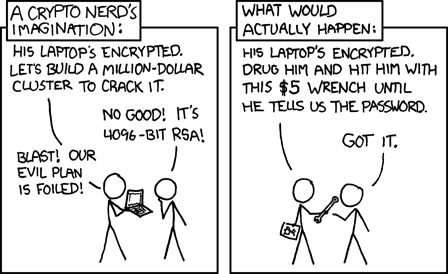
\includegraphics[width=10cm]{pictures_bitmap/security.png}\\
        \url{http://xkcd.com/538/} \href{http://creativecommons.org/licenses/by-nc/2.5/}{ Creative Commons Attribution-NonCommercial 2.5 License}.
\end{center}%
}{}             % Le gars de xkcd ne m'a pas encore répondu pour l'utilisation de l'image.

\noindent \ldots tout dépends du contexte.

